
\section{Theorie}
\label{sec:Theorie}

\subsection{Richardson-Gleichung}
Freie Elektronen in einem Leiter sind durch eine Potentialdifferenz $\phi$ zwischen dem Gebiet im Leiter und der Umgebung an diesem gebunden. Um diesen Leiter verlassen zu können muss ein Elektron eine genügend hohe Energie besitzen um die Differenz in den Potentialen überwinden zu können. Die Energieverteilung ist ist durch die Fermi-Diracsche Verteilungsfunktion 
\begin{equation}
	f(E) = \frac{1}{\exp\left(\frac{E-\zeta}{k T}\right)+1}
\end{equation} 
gegeben, wobei $\zeta$ die Fermische Grenzenergie, $T$ die Temperatur und $k$ die Boltzmann-Konstante ist. Diese Funktion ist in Abbildung \ref{fig:Fermi-Diracsche} skizziert. Es können nun alle Elektronen mit einer Energie größer als $\zeta + e_0 \phi$ mit einem Geschwindigkeitsvektor in Richtung der Oberflächennormalen den Leiter verlassen. Um den gesuchten aus dem Leiter austretenden Elektronenstrom zu ermitteln, wird die betrachtete Oberfläche $A$ mal die Geschwindigkeit der Elektronen $v$ in Richtung der Oberflächennormalen des Leiters mal die Zahl der Elektronen pro Volumen über alle Elektronen, welche den Leiter verlassen können, summiert. Dieses ist besonders gut im Phasenraum möglich und schließlich ergibt sich für den Sättigungsstrom $I_\text{S}$ die Richardson-Gleichung: 
\begin{equation}
	I_\text{S} = 4 \pi A e_0 m_0 \frac{k^2}{h^3} T^2 \exp\left(-e_0 \frac{\phi}{k T}\right)\text{.}
\end{equation}
\begin{figure}
	\centering
	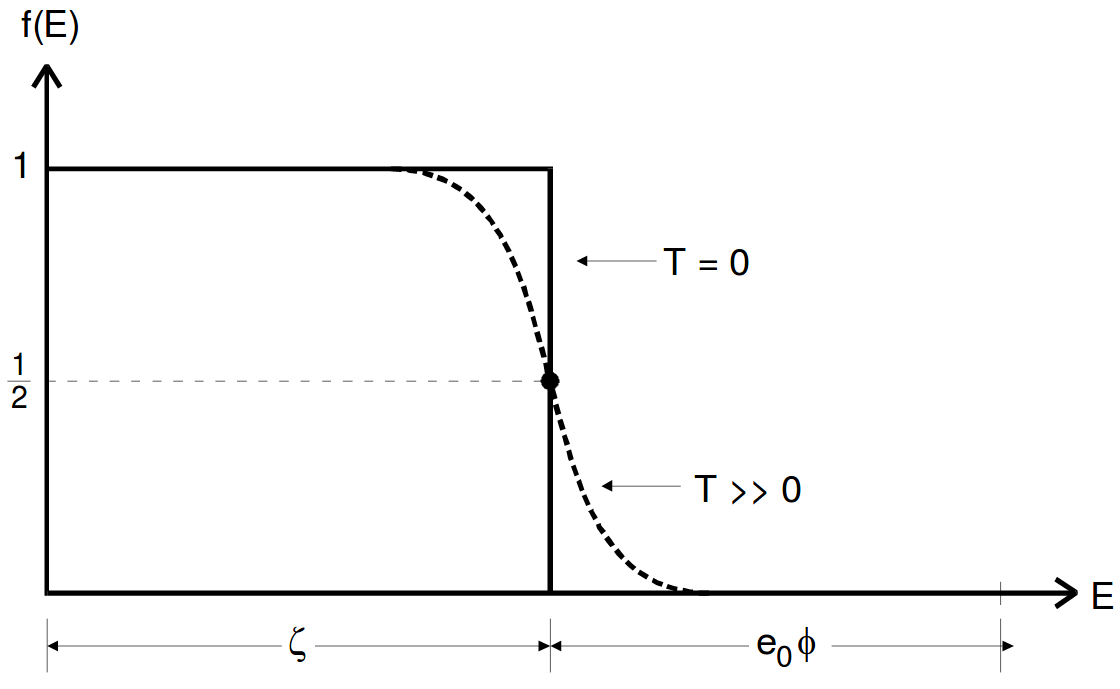
\includegraphics[width=\linewidth-100pt,height=\textheight-100pt,keepaspectratio]{content/Bilder/Fermi-Diracsche_Verteilung.png}
	\caption{Darstellung der Fermi-Diracschen Verteilungsfunktion für $T=0$ und $T\gg0$ \cite{V504}.}
	\label{fig:Fermi-Diracsche}
\end{figure}

\subsection{Hochvakuum-Diode}
Damit annähernd der Sättigungsstrom gemessen werden kann, dürfen die Elektronen nicht mit dem äußerem Medium wechselwirken und müssen zusätzlich nach dem Austritt abgesaugt werden. Dies wird bei einer Hochvakuum-Diode dadurch erreicht, indem zwischen der Kathode (dem Glühdraht) und der Anode eine Spannung angelegt wird und auch der Bereich dazwischen evakuiert wird. Die Diode ist in Abbildung \ref{fig:Hochvakuum-Diode} schematisch dargestellt.
\begin{figure}
	\centering
	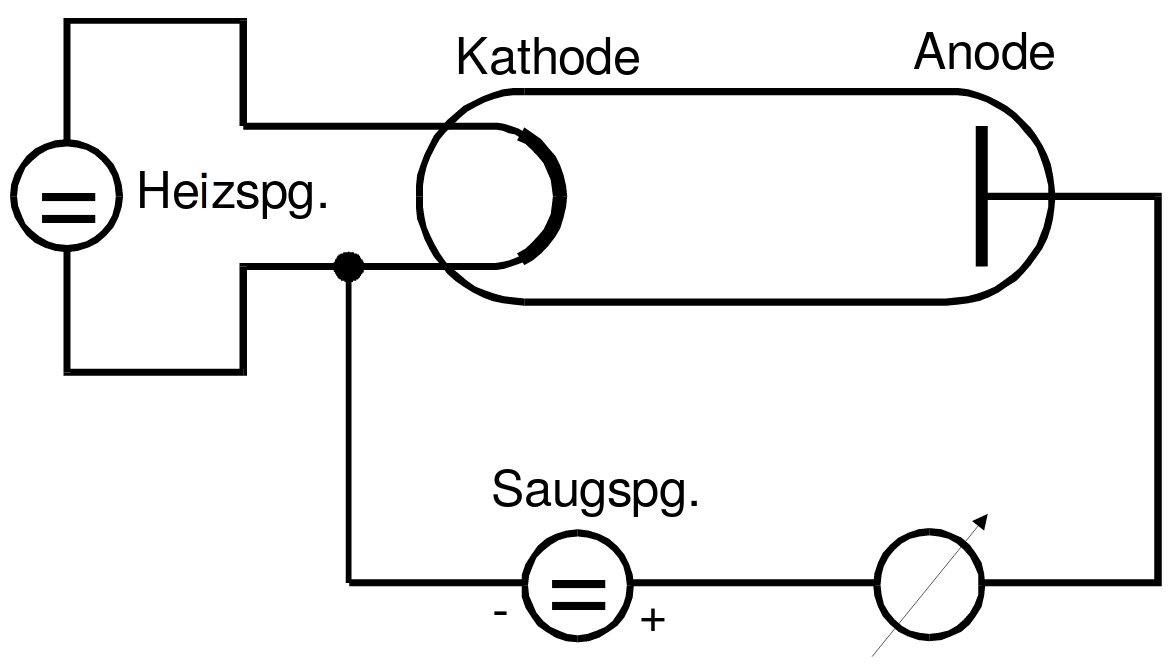
\includegraphics[width=\linewidth-100pt,height=\textheight-100pt,keepaspectratio]{content/Bilder/Hochvakuum-Diode.png}
	\caption{Grundlegende Darstellung einer Hochvakuum-Diode \cite{V504}.}
	\label{fig:Hochvakuum-Diode}
\end{figure}

\subsection{Langmuir-Schottkysche Raumladungsgleichung}
Da die Elektronen jedoch eine Beschleunigung in Richtung der Anode erfahren und der Strom überall konstant ist, folgt aus $I = -\rho v A $, dass die Ladungsverteilung zur Anode hin geringer werden muss. Diese Ladungshäufung vor der Kathode führt dazu, dass bei geringen Saugspannungen $V$, die Stromstärke $I$ unter dem Sättigungsstrom $I_\text{S}$ liegt und im Raumladungsgebiet annähernd durch die Langmuir-Schottkysche Raumladungsgleichung 
\begin{equation}
	I = \frac{4}{9} A e_0 \sqrt{2 e_0/m_0} \frac{V^\frac{3}{2}}{a^2} 
\end{equation} 
beschrieben wird. Der Abstand zwischen der Anode und der Kathode wird hier mit $a$ bezeichnet.

\subsection{Anlaufstrom bei einer anliegenden Gegenspannung an der Hochvakuums-Diode}
Die Elektronen können auch ohne eine anliegenden Spannung zwischen Kathode und Anode von der Kathode zur Anode wandern. Dies liegt daran, dass es Elektronen gibt, die eine größere Geschwindigkeit in Richtung der Oberflächennormalen besitzen, als zum Verlassen des Leiters notwendig wäre und sie somit nach dem Austreten noch eine Geschwindigkeit in Richtung Anode besitzen. Diese Geschwindigkeit entscheidet bis zu welcher Gegenspannung das Elektron noch an der Anode ankommt. Offensichtlich nimmt der Anlaufstrom mit wachsender Gegenspannung ab. Diese Anlaufstromstärke im Anlaufstromgebiet ist durch 
\begin{equation} 
	I = I_0 \exp\left(-\frac{e_0 (-V +\phi_A)}{k T}\right)
\end{equation}
gegeben. Hierbei ist $V\le0$ die Gegenspannung und $\phi_A e_0$ ist die Austrittsarbeit an der Anode.



\subsection{Kennlinie der Hochvakuum-Diode}
Eine Kennlinie einer Hochvakuums-Diode ist abhängig von der Temperatur an der Kathode. Bei größeren Temperaturen ist auch die Stromstärke bei der selben Saugspannung größer. Bei allen Kennlinien steigt die Stromstärke bei größer werdenden Saugspannungen. Die Kennlinie wird in drei Bereiche unterteilt. Der Bereich in welchem eine Gegenspannung ($V\le0$) anliegt, wird Anlaufstromgebiet genannt und zeichnet sich durch den exponentiellen Anstieg aus. Das anschließende Gebiet nennt sich Raumladungsgebiet und zeichnet sich durch $I \propto V^\frac{3}{2}$ aus. Das Sättigungsstromgebiet schließt sich daran an und zeichnet sich nun nicht mehr durch eine Proportionalität zu $V^\frac{3}{2}$ sondern durch eine asymptotische Annäherung an die Sättigungsstromstärke $I_\text{S}$ aus. Eine solche Kennlinie ist in Abbildung \ref{fig:Kennlinie} zu sehen.
\begin{figure}
	\centering
	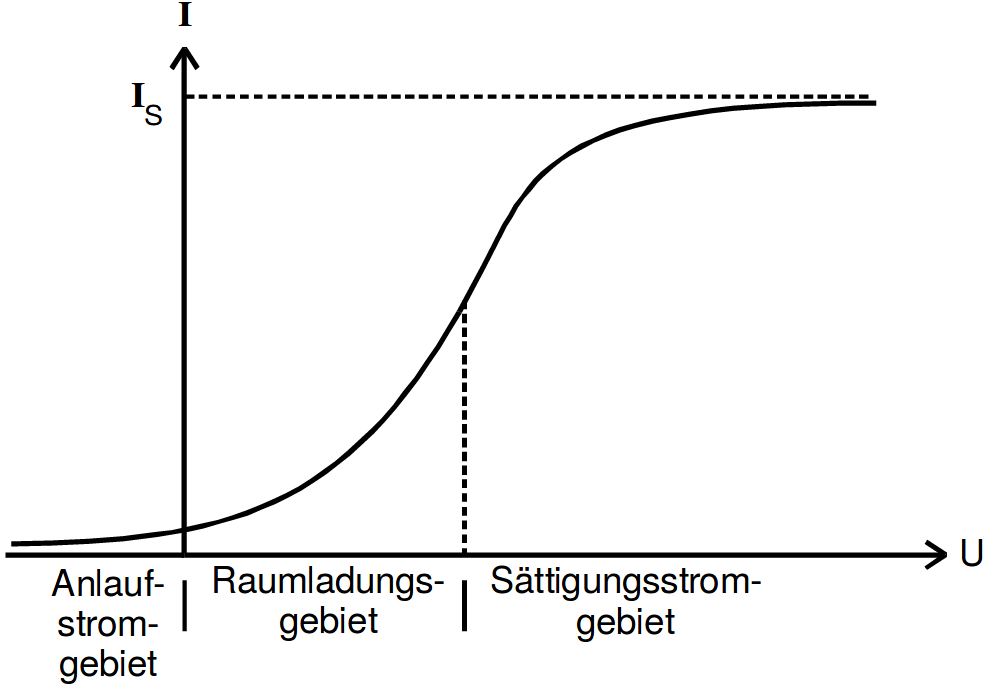
\includegraphics[width=\linewidth-100pt,height=\textheight-100pt,keepaspectratio]{content/Bilder/Kennlinie.png}
	\caption{Mögliche Kennlinie einer Hochvakuums-Diode \cite{V504}.}
	\label{fig:Kennlinie}
\end{figure}

